\chapter{Określanie lokalizacji}
\label{cha:lokalizacja}
\section{Lokalizacja użytkownika}
Lokalizacja użytkownika w systemie określa się na podstawie odległości od punktów, których współrzędne w przestrzeni trójwymiarowej są znane. Są to głównie routery i Beacony, jednak może się zdarzyć, że takim punktem staje się również inny użytkownik. Współrzędne użytkownika można obliczyć, podając siły sygnałów odebranych przez otaczające go urządzenia i obliczając na ich podstawie dystans.
\section{Trilateracja}
Najbardziej znanym sposobem obliczenia lokalizacji użytkownika na podstawie dystansu do znanych punktów jest trilateracja. Metoda ta polega na przedstawienie dystansu dzielącego punkt od nadajników jako okręgi (lub jako sfery w przypadku, gdy określamy lokalizację w trzech wymiarach). Następnie, należy wyznaczyć współrzędne punktu przecięcia okręgów. Wyznaczone współrzędne są lokalizacją punktu, dla którego dokonywaliśmy obliczenia.
\begin{figure}[H]			
	\centering
	\caption{Wizualizacja modelu trilateracji}
	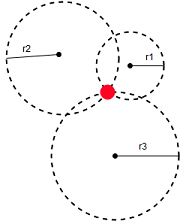
\includegraphics{trilateracja}
\end{figure}
Współrzędną punktu można obliczyć na podstawie wzoru:
\begin{equation}
\left\{
\begin{array}{l}
(x_p-x_1)^2 + (y_p - y_1)^2 = r_1^2\\
(x_p-x_2)^2 + (y_p - y_2)^2 = r_2^2\\
(x_p-x_3)^2 + (y_p - y_3)^2 = r_3^2
\end{array}
\right.
\end{equation}
gdzie:
\begin{itemize}
	\item $x_p$, $y_p$ to współrzędne obliczanego punktu
	\item $x_1$, $y_1$, $x_2$, $y_2$, $x_3$, $y_3$ to współrzędne znanych punktów
	\item $r_1$, $r_2$, $r_3$ to odległości między punktem obliczanym, a punktami o znanych współrzędnych
\end{itemize}
Ta metoda lokalizowania użytkownika w przestrzeni ma jedną, bardzo ważną wadę, która wyklucza jej wykorzystanie w stworzonym systemie - nie potrafi się dostosować do błędów pomiarów, których w przypadku określania lokalizacji przy użyciu sygnałów radiowych, jest dużo. Aby obliczane lokalizację użytkowników w sposób zbliżony odwzorowywały rzeczywiste położenie, algorytm obliczający musiał być bardziej odporny na błędy pomiarowe.
\section{Lokalizacja jako funkcja probabilistyczna Gaussa}
\subsection{Funkcja Gaussa}